\documentclass[10pt,landscape]{article}
\usepackage{multicol}
\usepackage{calc}
\usepackage{ifthen}
\usepackage[landscape]{geometry}
\usepackage{hyperref}
\usepackage{amsmath,amsfonts}
\usepackage{blkarray,booktabs}
\usepackage{enumitem}
\usepackage{graphicx}
\usepackage{makecell}
\usepackage{tabularx}
%wholesome

% To make this come out properly in landscape mode, do one of the following
% 1.
%  pdflatex latexsheet.tex
%
% 2.
%  latex latexsheet.tex
%  dvips -P pdf  -t landscape latexsheet.dvi
%  ps2pdf latexsheet.ps


% To Do:
% \listoffigures \listoftables
% \setcounter{secnumdepth}{0}


% This sets page margins to .5 inch if using letter paper, and to 1cm
% if using A4 paper. (This probably isn't strictly necessary.)
% If using another size paper, use default 1cm margins.
\ifthenelse{\lengthtest { \paperwidth = 11in}}
	{ \geometry{top=0.1in,left=0.1in,right=0.1in,bottom=0.1in} }
	{\ifthenelse{ \lengthtest{ \paperwidth = 297mm}}
		{\geometry{top=1cm,left=1cm,right=1cm,bottom=1cm} }
		{\geometry{top=1cm,left=1cm,right=1cm,bottom=1cm} }
	}

\DeclareMathOperator*{\Uniform}{Uniform}
\DeclareMathOperator*{\bias}{bias}
\DeclareMathOperator*{\rank}{rank}
\DeclareMathOperator*{\Row}{Row}
\DeclareMathOperator*{\Var}{Var}
\DeclareMathOperator*{\Cov}{Cov}
\DeclareMathOperator*{\trace}{Tr}
\DeclareMathOperator*{\argmax}{argmax}
\DeclareMathOperator*{\argmin}{argmin}
\DeclareMathOperator*{\supp}{supp}
\newcommand{\innerprod}[2]{\langle #1, #2 \rangle}
\newcommand{\deriv}[2]{\frac{\d #1}{\d #2}}
\newcommand{\pderiv}[2]{\frac{\partial #1}{\partial #2}}
% \newcommand{\pd}[2]{\frac{\partial{#1}}{\partial{#2}}}
\newcommand{\wrap}[3]{\left#1#3\right#2}
\newcommand*{\Scale}[2][4]{\scalebox{#1}{$#2$}}%
\def\d{ \, \mathrm{d}}
\def\P{\mathbb{P}}
\def\E{\mathbb{E}}


% Turn off header and footer
\pagestyle{empty}
 

% Redefine section commands to use less space
\makeatletter
\renewcommand{\section}{\@startsection{section}{1}{0mm}%
                                {-1ex plus -.5ex minus -.2ex}%
                                {0.5ex plus .2ex}%x
                                {\normalfont\large\bfseries}}
\renewcommand{\subsection}{\@startsection{subsection}{2}{0mm}%
                                {-1explus -.5ex minus -.2ex}%
                                {0.5ex plus .2ex}%
                                {\normalfont\normalsize\bfseries}}
\renewcommand{\subsubsection}{\@startsection{subsubsection}{3}{0mm}%
                                {-1ex plus -.5ex minus -.2ex}%
                                {1ex plus .2ex}%
                                {\normalfont\small\bfseries}}
\makeatother

% Define BibTeX command
\def\BibTeX{{\rm B\kern-.05em{\sc i\kern-.025em b}\kern-.08em
    T\kern-.1667em\lower.7ex\hbox{E}\kern-.125emX}}

% Don't print section numbers
\setcounter{secnumdepth}{0}


\setlength{\parindent}{0pt}
\setlength{\parskip}{0pt plus 0.5ex}


% -----------------------------------------------------------------------

\begin{document}

\raggedright
\footnotesize
\begin{multicols}{3}


% multicol parameters
% These lengths are set only within the two main columns
%\setlength{\columnseprule}{0.25pt}
\setlength{\premulticols}{1pt}
\setlength{\postmulticols}{1pt}
\setlength{\multicolsep}{1pt}
\setlength{\columnsep}{2pt}

% \begin{center}
%      \Large{\textbf{CS 189 Cheat Sheet}} \\
% \end{center}

\section{$\boxed{\text{Classification}}$}


\subsection{\textit{k}-Nearest Neighbors}
kNNs are bounded by $\leq 2$x the Bayes optimal error, $N,k\to\infty, k/N\to0$.
\newlength{\MyLen}
\settowidth{\MyLen}{\texttt{letterpaper}/\texttt{a4paper} \ }
\begin{tabular}{@{}p{\the\MyLen}%
                @{}p{\linewidth-\the\MyLen}@{}}
Edge Case & 2 pts w/ same features but diff classes.
\\
Robustness & Generalizes better to test data.
\\
Fit & Better training classification. \\
Validation & Hold back data subset as validation set.
\\
& Train multiple times w/ diff hyperparams.
\\
& Choose what is best on validation set.
\\
Training Set & Used to learn model weights.\\
Validation Set & Tunes hyperparameters (ex. $k\in$  $k$NN).\\
Test Set & used as FINAL evaluation of model.\\
Isocontour of $f$ & $L_{c}=\{x \mid f(x)=c\}$, with isovalue $c$.\\
Isotropic Gaussian & Same var in ea dir: $\Sigma=cI$.\\
Anisotropic Gaussian & Allows diff amnts of var along diff dirs, $\Sigma\succ 0$.
\end{tabular}

\subsection{Perceptron}
Model/rule: 1 if $\vec{X_i}\cdot \vec w\geq0$ elif $\vec{X_i}\cdot \vec w\leq0\implies$ -1.

Loss: $L(z, y_{i})=0$ if $y_{i} z \geq 0$ else $-y_{i} z$, ($z$=pred, $y_i$=true ans).

$R(w)=\displaystyle\sum_{i=1}^{n} L\left(X_{i} \cdot w, y_{i}\right)=\sum_{i \in V}-y_{i} X_{i} \cdot w$
\\
Gives some linear boundary; if data is linearly separable, correctly classifies all data in at most $O\left(\frac{r^2}{\gamma^2}\right)$ iterations.

\subsection{Support Vector Machines}
Hard-Margin: $\displaystyle\min_{\vec w, b}\|\vec w\|_2^2$, 
\ s.t. $y_i(\vec w^\top\vec{x_i}-b)\geq1 \ \forall i$
\\
{\scriptsize{Fails w/ non-linearly sep. data. Margin size = $\frac{1}{\|w \|}$, Slab size = $\frac{2}{\|w\|}$}}
\begin{tabular}{@{}ll@{}}
Hyperplane & $H=\{x:w\cdot x=-\alpha\}$\\
& flat, infinite, $\dim(d-1)$ plane\\
$x, y\in H$ & $\vec w\cdot(y-x)=0, \vec w$ is normal vec of $H$.
\\
Support Vectors & Examples needed to find $f(\mathbf x)\in$ SVM. \\
                   & Examples with non-0 weight $\alpha_k\in$ SVM. \\
\end{tabular}

\subsection{Soft-Margin}
Allows misclassifications:
$\min_{\vec w, b, \xi_i}\frac12\|\vec w\|^2+C\sum_{i=1}^n \xi_i$ s.t. \vspace{-0.1cm}\begin{align*}
    y_i(\vec w^\top \vec{x_i}-b)\geq1-\xi_i, \ \ \forall i;\quad
    \xi_i\geq 0, \quad\forall i
\end{align*}
Small C: maximize margin, underfitting, less sensitive, more flat. \\
Big C: minimize margin, overfitting, very sensitive, more sinuous.
\\
$C\to\infty\implies$ Soft-Margin $\to$ Hard-Margin. Note $C\geq0$.

\subsection{Generative}
Want to learn \textbf{everything} about data before you classify: \\
the \textbf{priors} $\hat\pi_i=\Pr(Y=C_i)$ and \textbf{cond. dist} $\mathbb{P}(X|Y=C_i)$.
\textbf{Posterior}: $\mathbb{P}(Y=C_i | X) = \frac{\mathbb{P}(X \mid Y = C_i) \cdot \mathbb{P}(Y=C_i)}{\mathbb{P}(X)}$ 
\settowidth{\MyLen}{-\texttt{multicol} }
\begin{tabular}{@{}p{\the\MyLen}%
                @{}p{\linewidth-\the\MyLen}@{}}
%\begin{tabular}{@{}ll@{}}
Logistic Function: & $\frac{1}{1 + e^{-h(x)}}, $ where $h(x)$ is \textbf{linear} in terms of features. True in LDA but not QDA (where $h(x)$ is quadratic).\\
GDA: & Assumes each class models a Gaussian distribution. \\
QDA:  &  Works with any number of classes; $\frac{d(d+3)}{2}+1$ params.\\
LDA:  &  when variances are equal; $d+1$ params.\\
\end{tabular}
Isotropic:\\
\quad QDA: $\widehat{\sigma }^2 = \frac{1}{dn} \sum_{i : y_i = C}^{} \left \| x_i - \widehat{\mu _c} \right \|^2$\\
\quad LDA: $\widehat{\sigma }^2 = \frac{1}{dn} \sum_{C}^{}\sum_{i : y_i = C}^{} \left \| x_i - \widehat{\mu _c} \right \|^2$\\

Anisotropic:\\
\quad QDA: $\widehat{\Sigma}_c = \frac{1}{n_c} \sum_{i : y_i = C}^{} (X_i - \widehat{\mu _c})(X_i - \widehat{\mu _c})^\top$\\
\quad LDA: $\widehat{\Sigma} = \frac{1}{n} \sum_{C}^{}\sum_{i : y_i = C}^{} (X_i - \widehat{\mu _c})(X_i - \widehat{\mu _c})^T$ \\ \vspace{8mm}
Choose $C$ to maximize discriminant: \\ QDA: $Q_C=-\frac{1}{2}\left(x-\mu_{\mathrm{C}}\right)^{\top} \Sigma_{\mathrm{C}}^{-1}\left(x-\mu_{\mathrm{C}}\right)-\frac{1}{2} \ln \left|\Sigma_{\mathrm{C}}\right|+\ln \pi_{\mathrm{C}}$ \\ LDA: $Q_C=\mu_{\mathrm{C}}^{\top} \Sigma^{-1} x-\frac{\mu_{\mathrm{C}}^{\top} \Sigma^{-1} \mu_{\mathrm{C}}}{2}+\ln \pi_{\mathrm{C}}$
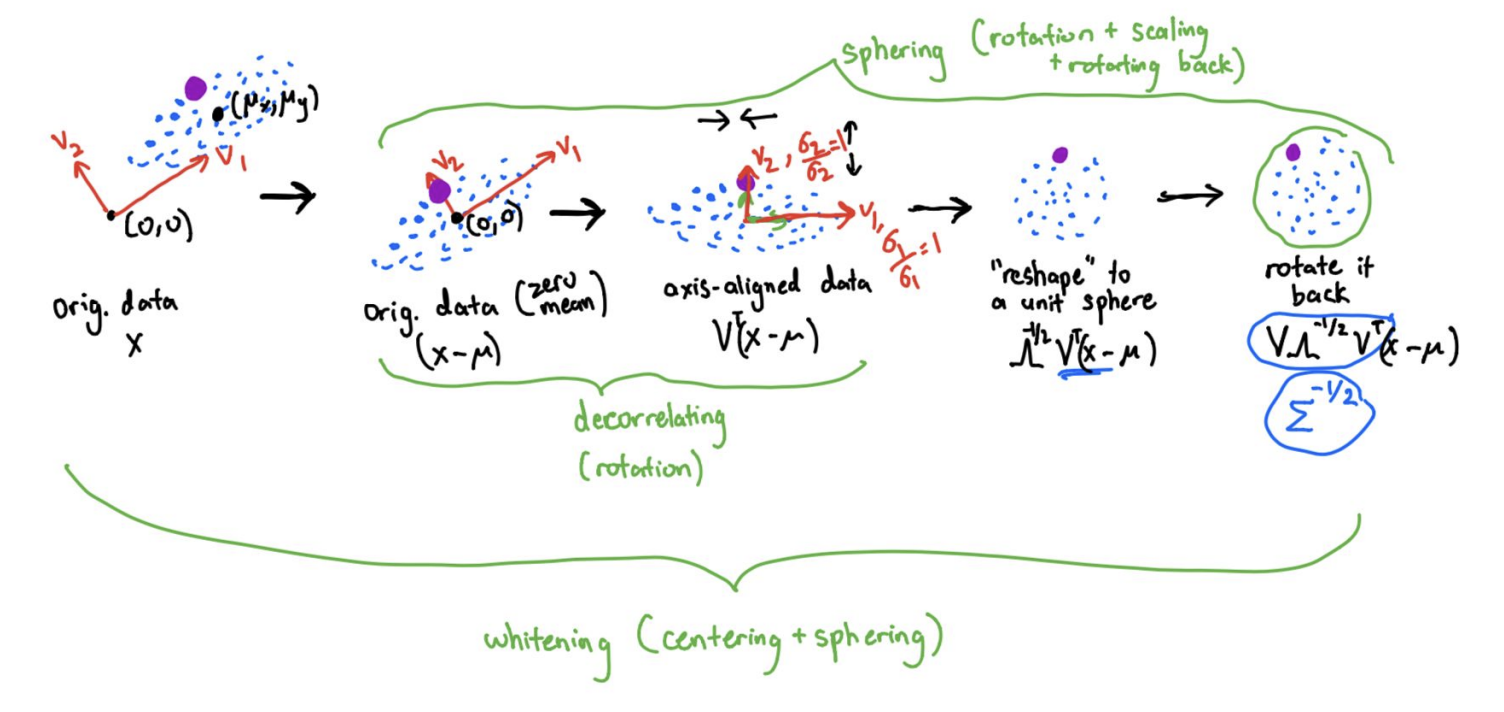
\includegraphics[width=90mm]{whitening.png}
\subsection{Discriminative}
Want to learn a \textit{few} things before trying to classify.\\
Only tries to model $\P(Y|X)$ from training data.\\
\textbf{Logistic Reg} (2 classes):
For a training point, $P\left(Y=y_{i} \mid x\right)=p^{y_{i}}(1-p)^{1-y_{i}}$. Note that $p=s\left(w^{T} x\right)$ as given by our model of the posterior $P(Y=1 \mid x)$. MLE on this leads to the cross entropy loss function (which is convex!), namely
$$
L(w)=-\sum \Big(y_{i} \ln p_{i}+\left(1-y_{i}\right) \ln \left(1-p_{i}\right)\Big)
$$
Note: $P(Y=1 \mid x)=\frac{1}{1+\exp \left(-w^{T} x\right)}$; $s^{\prime}(\gamma) = s(\gamma)(1 - s(\gamma))$ \\
\text{Sigmoid Function}: 
$s(\gamma) = \frac{1}{1 + e^{-\gamma}}$
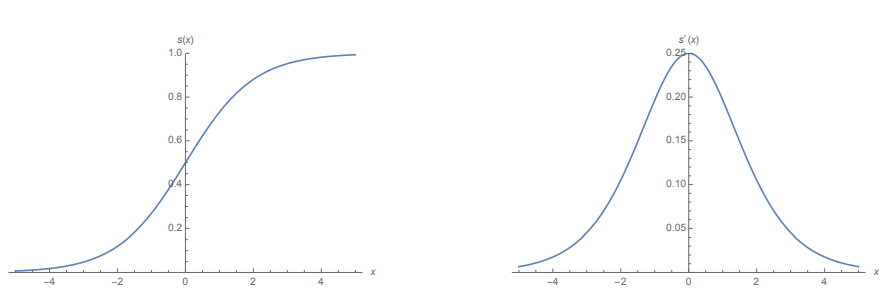
\includegraphics[width=\linewidth, height = 1.7 in]{Sigmoid1.png}
Decision Boundary: of the form $w^{T} x>c_{1}$ thus must be linear. Though probability predictions are non-linear, actual boundary is linear. Log Reg always separates linearly separable points. \\
\textbf{Softmax Reg:} logistic regression for multiple classes 



\section{$\boxed{\text{Probability}}$}
\textbf{Multivariate Gaussian PDF:}\\
$f_{\mathbf{X}}\left(x_{1}, \ldots, x_{k}\right)=\frac{\exp \left(-\frac{1}{2}(\mathbf{x}-\boldsymbol{\mu})^{\mathrm{T}} \boldsymbol{\Sigma}^{-1}(\mathbf{x}-\boldsymbol{\mu})\right)}{\sqrt{(2 \pi)^{k}|\mathbf{\Sigma}|}}$
\subsection{MLE (Maximum Likelihood Estimate)}
We have $A, B, C, D$. 
$P(A \mid B) > P(A \mid C) > P(A \mid D)\newline\implies B$ is the MLE of $A$. MLE Estimate of Anisotropic can be PSD.

$\hat{\theta}_{MLE}(x) = \underset{\theta}{\text{arg max}} \ \Pi f(x \mid \theta) = \underset{\theta}{\text{arg max}} \ln\mathcal{L}(\theta; x)$  \\
Mean is unbiased; Variance is biased (usually underestimate)\\

Predicts parameter which max the probability
of the data.
Implicitly assumes uniform prior
\vspace{-0.25em}
\subsection{MAP (Maximum a Posteriori)}
We have $A, B, C, D$. 
$\P(A \mid B) > \P(C \mid B) > \P(D \mid B)\newline\implies A$ is the MAP of $B$.

$\hat{\theta}_{MAP} = \underset{\theta}{\text{arg max}} f(\theta \mid x) = \underset{\theta}{\text{arg max}} f(x \mid \theta) \cdot g(\theta)$ \\

Predicts the parameter which maximizes the conditional
probability of the parameter given the data.
\\
Should be used when you have the prior probabilities.

MLE = MAP when all parameters have equal prior probability.
\\
The axis lengths of Gaussian Isocontours are $\sigma_i$ s.t. $\sigma^2(X)=\Var(X)$.
Independent $\Longleftrightarrow$ uncorrelated (only for MVGs).




\subsection{Bayesian Risk}
$L$ (loss function) is symmetric: pick class with max posterior prob.
\\
$L$ is asymmetric: minimize $\E[L(\text{true class}, \text{prediction}) \mid \text{data}]$ or pick max loss-weighted posterior prob.
\\

The risk for $r$ is the expected loss over all values of $x, y$. Equals to 0 when class distros don't overlap or prior prob for one class is 1. Let $C$ be the set of classes $Y$ can take.
{
  \begin{align*}
    R(r) &=\E[L(r(X), Y)] \\
    &=\sum_{x}\wrap(){\sum_{c\in C} L(r(x), c) P(Y=c \mid X=x)} P(X=x) \\
    &=\sum_{c\in C}\wrap(){ P(Y=c) \sum_{x} L(r(x), c) P(X=x \mid Y=c)} \\
    &= R(\hat{y}=i \mid x)=\sum_{j=1}^{n} \lambda_{i j} P(Y=j \mid x)
  \end{align*}
}
The Bayes decision rule aka Bayes classifier is the fn $r^{*}$ that minimizes functional $R(r)$. Assuming $L(z, y)=0$ for $z=y$:
{\scriptsize \[
r^{*}(x)=\left\{\begin{aligned}
1 & \text { if } L(-1,1) P(Y=1 \mid X=x)>L(1,-1) P(Y=-1 \mid X=x) \\
-1 & \text { otherwise }
\end{aligned}\right.
\]}
%---------------------------------------------------------------------------
% \newcommand{\FontCmd}[3]{\PBS\verb!\#1{!\textit{text}\verb!}!  \> %
%                          \verb!{\#2 !\textit{text}\verb!}! \> %
%                          \#1{#3}}
% \begin{tabular}{@{}l@{}l@{}l@{}}
% \textit{Command} & \textit{Declaration} & \textit{Effect} \\
% \verb!\textrm{!\textit{text}\verb!}!                    & %
%         \verb!{\rmfamily !\textit{text}\verb!}!               & %
%         \textrm{Roman family} \\
% \verb!\textsf{!\textit{text}\verb!}!                    & %
%         \verb!{\sffamily !\textit{text}\verb!}!               & %
%         \textsf{Sans serif family} \\
% \verb!\texttt{!\textit{text}\verb!}!                    & %
%         \verb!{\ttfamily !\textit{text}\verb!}!               & %
%         \texttt{Typewriter family} \\
% \verb!\textmd{!\textit{text}\verb!}!                    & %
%         \verb!{\mdseries !\textit{text}\verb!}!               & %
%         \textmd{Medium series} \\
% \verb!\textbf{!\textit{text}\verb!}!                    & %
%         \verb!{\bfseries !\textit{text}\verb!}!               & %
%         \textbf{Bold series} \\
% \verb!\textup{!\textit{text}\verb!}!                    & %
%         \verb!{\upshape !\textit{text}\verb!}!               & %
%         \textup{Upright shape} \\
% \verb!\textit{!\textit{text}\verb!}!                    & %
%         \verb!{\itshape !\textit{text}\verb!}!               & %
%         \textit{Italic shape} \\
% \verb!\textsl{!\textit{text}\verb!}!                    & %
%         \verb!{\slshape !\textit{text}\verb!}!               & %
%         \textsl{Slanted shape} \\
% \verb!\textsc{!\textit{text}\verb!}!                    & %
%         \verb!{\scshape !\textit{text}\verb!}!               & %
%         \textsc{Small Caps shape} \\
% \verb!\emph{!\textit{text}\verb!}!                      & %
%         \verb!{\em !\textit{text}\verb!}!               & %
%         \emph{Emphasized} \\
% \verb!\textnormal{!\textit{text}\verb!}!                & %
%         \verb!{\normalfont !\textit{text}\verb!}!       & %
%         \textnormal{Document font} \\
% \verb!\underline{!\textit{text}\verb!}!                 & %
%                                                         & %
%         \underline{Underline}
% \end{tabular}
\section{$\boxed{\text{Regression Methods}}$}
Model: $y = Xw$, Loss Function: least squares, $n \in N(X)$
\vspace{-0.5cm}
% \begin{center}
    \begin{tabular}{||c c p{0.3\linewidth}||} 
         \hline
         Name & Objective & Solution \\
         \hline
         \rule{0pt}{3ex}
         OLS & {\scriptsize $\frac1n\|Y-Xw\|_2^2$} & {\scriptsize $w^\ast=(X^\top X)^{\dagger} X^\top y \in X^{\dagger}y + n$} \\[0.4em] 
         \hline
         \rule{0pt}{3ex}
         \makecell{Ridge: Assumes \\Gaussian Priors} & {\scriptsize $\frac1n\|Y-Xw\|_2^2+\lambda \| w \|_2^2$} & {\scriptsize $w^\ast=(X^\top X + n\lambda I)^{-1} X^\top y$} \\[0.4em] 
         \hline
         \rule{0pt}{3ex}
         LASSO & {\scriptsize $\frac1n\|Y-Xw\|_2^2+\lambda \| w \|_1$} & No closed form \\ [1ex] 
         \hline
    \end{tabular}
% \end{center}
\vspace{0.3cm}


\section{$\boxed{\text{Linear Algebra}}$}
\subsection{Matrix Calculus}

\settowidth{\MyLen}{\texttt{.begin.verbatim..} }
\begin{tabular}{@{}p{\linewidth/2}%
                @{}p{\linewidth/2}@{}}
$\nabla_{\vec x}{\vec w^\top \vec x} = \wrap(){\pderiv{\vec w^\top \vec x}{\vec x}}^\top = \vec{w}$ & $\nabla_{\vec x}{(\vec w^\top A\vec x)}= A^{\top}\vec w$ \\
\hrule&\hrule\\
$\nabla_{A}{\vec w^\top A\vec x}=\vec w\vec x^\top$ & $\nabla_{\vec x}{(\vec x^\top A\vec x)} = (A+A^\top)\vec x$ \\
\hrule&\hrule\\
$\nabla_{\vec x}^2{(\vec x^\top A\vec x)} = A+A^\top$ & $\nabla_{\vec x}{(\alpha \vec{y})} = (\nabla_{\vec x}{\alpha})\vec{y}^{\top} + \alpha \nabla_{\vec x}{\vec y}$ \\
\hrule&\hrule
\\
$\nabla_{\vec x}{\vec{f}(\vec y)} = (\nabla_{\vec x}{\vec y})(\nabla_{\vec y}{\vec{f}(\vec y)})$ & $\nabla_{\vec x}(\vec{y} \cdot \vec{z}) = (\nabla_{\vec x}{\vec y})\vec{z}+(\nabla_{\vec x}{\vec z})\vec{y}$ \\
\hrule & \hrule
\\
$\nabla_{\vec x}{C\vec y(\vec{x})} = (\nabla_{\vec x}{\vec y(\vec x)})C^\top$ & $\pderiv{\|\vec x\|_2^2}{\vec x}=\pderiv{(\vec x^\top\vec x)}{\vec x}=2\vec x$ \\
\hrule&\hrule
\end{tabular} \vspace{-0.1cm}
$$\nabla_{\vec{y}} (\vec{y} - A \vec{x})^{\top} W(\vec{y} - A \vec{x}) = 2W(\vec{y} - A \vec{x})$$ \\
\hrule
$$\nabla_{\vec{x}} (\vec{y} - A \vec{x})^{\top} W(\vec{y} - A \vec{x}) = -2A^{\top}W(\vec{y} - A \vec{x})$$  \\
\hrule
$$\nabla_{\vec w} \wrap(){\|X\vec w-\vec y\|_2^2+\lambda\|\vec w\|_2^2} = 2X^\top X\vec w-2X^\top \vec y+2\lambda\vec w$$
\hrule

\subsection{Matrix $A$ is \underline{Positive Semi-Definite} iff}
\begin{enumerate}[label=(\alph*)]
    \item $\forall \vec x \neq \vec{0} \in \mathbb{R}^{n}, \vec x^{\top} A \vec x \geq 0$. Symmetric.
    \item All eigenvalues of $A$ are non-negative ($\lambda_i\ge0$).
    \item $\exists$ unique matrix $L \in \mathbb{R}^{n \times n}$ such that $A=L L^{\top}$ (Cholesky decomposition).
\end{enumerate}
PSD Example: $A=\begin{bmatrix}2&-1\\-1&2\end{bmatrix}$, with $\lambda=3,1$. $L=\begin{bmatrix}1&0\\-1&1\end{bmatrix}$.
\\
All diagonal entries of A are non-negative and $\trace(A)\geq0$. \\
Sum of all the entries $\geq0$. $\Var(Mx) = M\Var(x)M^T, M$ is constant.
$M\succ0, N\succ0, M-N\succeq0\implies N^{-1}-M^{-1}\succeq0$\\
$M\succeq0, N\succeq0\implies M-N\succeq0\iff\lambda_{\min}(M)>\lambda_{\max}(N)$.\\
$A = A^{\frac{1}{2}}A^{\frac{1}{2}}=U \Lambda^{\frac{1}{2}}\Lambda^{\frac{1}{2}}U^{\top}$, $A^{\frac{1}{2}} = U \Lambda^{\frac{1}{2}}U^{\top}$  \\
A function is convex iff Hessian is PSD. Strict Convexity: $(\forall 0<t<1), f(tx_1+(1-t)x_2)<tf(x_1)+(1-t)f(x_2)$

\textbf{Covariance Matrix}
$\begin{aligned}[t]\Sigma &=\frac{1}{n}\hat{X}^{\top}X = 
%\begin{blockarray}{cc}
%\begin{block}{[cc]}
%\Var(x) & \Cov(x, y) \\
%\Cov(x, y) & \Var(y)\\
%\end{block}
%\end{blockarray}\vspace*{-1.25\baselineskip}
{\tiny\begin{bmatrix}
\Var(X_1) & \Cov(X_1, X_2) & \cdots &  \Cov(X_1, X_d) \\
\Cov(X_2, X_1) & \Var(X_2) & \cdots & \Cov(X_2, X_d) \\
\vdots & \vdots & \ddots & \vdots \\
\Cov(X_d, X_1) & \Cov(X_d, X_2) & \cdots & \Var(X_d)
\end{bmatrix}} \\
&= \E[(X - \mu)^{\top}(X - \mu)] \text{ where } X \in \mathbb{R}^{n \times d} \text{, all diag entries $>$ 0}
\end{aligned}$
\\ \vspace{0.1cm}
 Symmetric, PSD $\implies\exists \Sigma=V\Lambda V^\top$ by Spectral Theorem.
PD $\implies$ symmetric in this class. Eigenvectors are orthogonal directions along which points are uncorrelated. $\Sigma^{-1} = V \Lambda^{-1}V^{\top} = \sum_i \frac{1}{\Lambda_{ii}}v_iv_i^{\top}$

\textbf{Spectral Theorem: }$A=V\Lambda V^\top$.
All real+symmetric $n \times n$ matrices have real eigenvalues and $n$ eigenvectors that are mutually orthogonal: $v_{i}^{\top} v_{j}=0 \quad  \forall i \neq j$.

\subsection{Norm Ball}
$\ell_0$ and $\ell_1$ encourage sparsity (more than $\ell_2$).
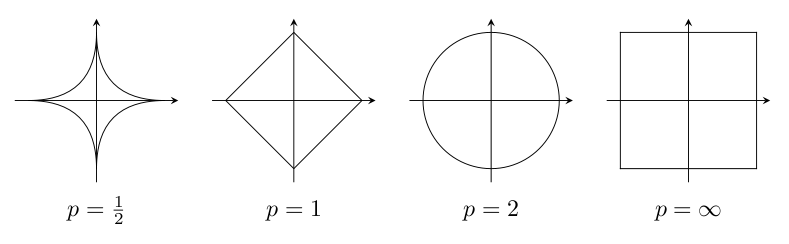
\includegraphics[scale=0.2]{norms.png}

\subsection{Fundamental Theorem of Linear Algebra}
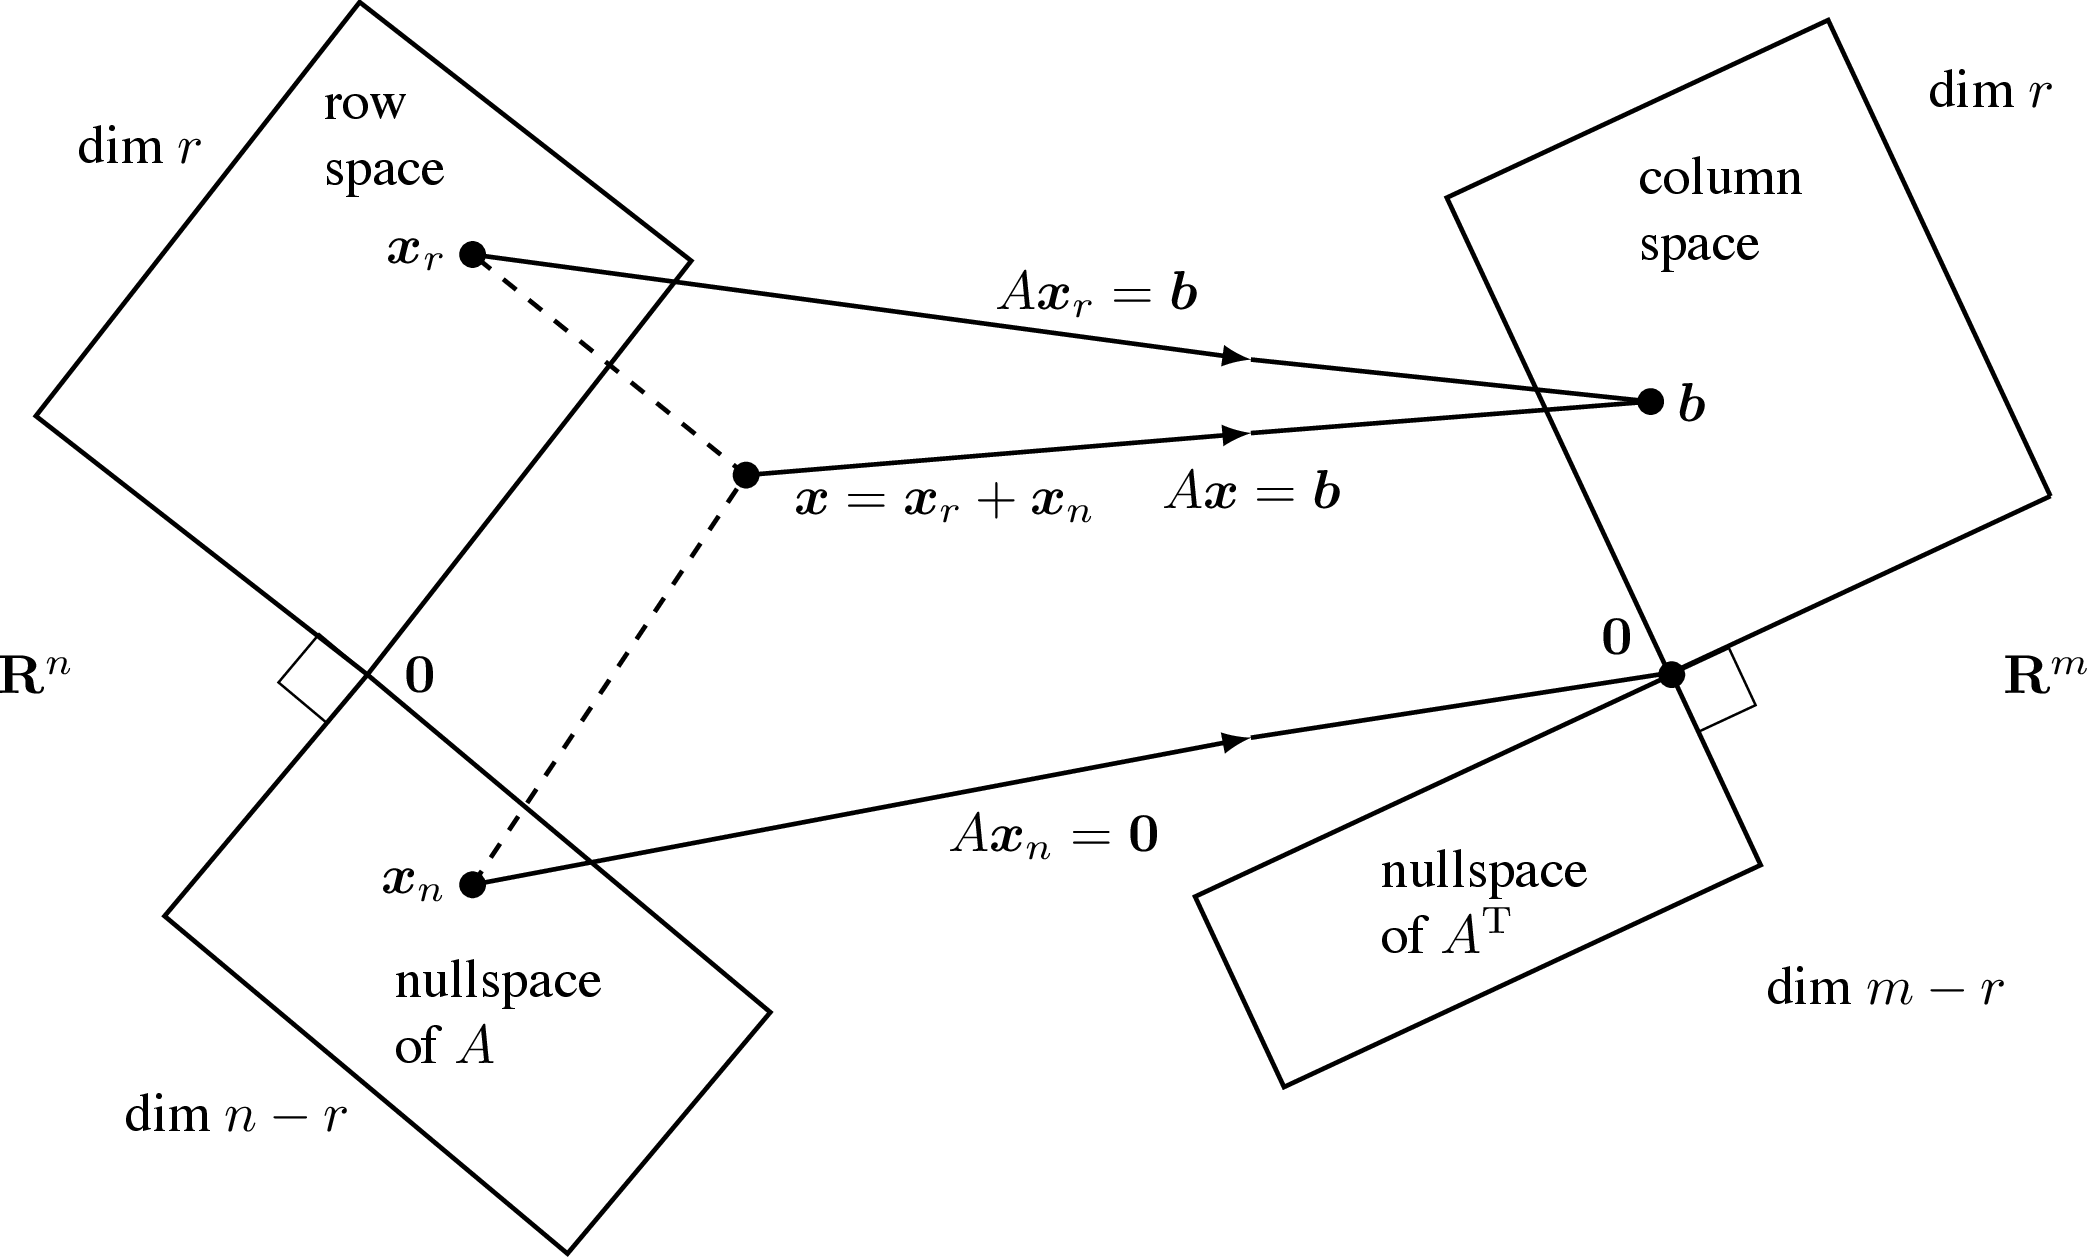
\includegraphics[scale=0.1]{strang.png}\\
$\small{(N(A)^{\perp} = R(A^{\top})) \oplus (N(A^\top A)=N(A) = R(A^{\top})^{\perp}) = \mathbb{R}^n}$ \\
    $(N(A^{\top})^{\perp} = R(A)) \oplus (N(A^{\top}) = R(A)^{\perp}) = \mathbb{R}^m$ \\
Rank-nullity Theorem: dim($R(A)$) + dim($N(A)$) = $n$
\\
Jensen's Inequality: If $f(x)$ is strictly convex, $\E[f(x)]>f(\E[x])$.
\\
$\dim(\Row(X))=\dim(R(X^\top))=\rank(X^\top)=\rank(X)$.
$\Row(X^\top X)=R(X^\top X)=\Row(X)=R(X^\top)$
\section{$\boxed{\text{Update Rule}}$}

% \subsection{Font face}
\settowidth{\MyLen}{\texttt{.begin.verbatim..} }
\begin{tabular}{@{}p{\the\MyLen}%
                @{}p{\linewidth-\the\MyLen}@{}}
Gradient Descent: & $w^{(t+1)} \leftarrow w^{(t)} - \eta \nabla_w J(w^{(t)}) $ \\
Logistic Reg:& $w^{(t+1)} \leftarrow w^{(t)} + \epsilon X^{\top}\wrap(){y - s(Xw^{(t)})}$ \\
\hrule&\hrule\\
Newton's Method: & $w^{(t+1)} \leftarrow w^{(t)} - (\nabla^2_w J(w^{(t)}))^{-1} \nabla_w J(w^{(t)})$ \\
*** Note: & If $J$ quadratic, Newton's method only needs one step to find exact solution. Newton's Method doesn't work for most nonsmooth functions, and is generally faster than BGD/SGD. \\
\hrule&\hrule\\
Stochastic GD: & $w \leftarrow w - \epsilon \nabla_w J(w)_i$ for some $i \in U([1, \dots, n])$ \\
Logistic Reg: & $w \leftarrow w + \epsilon (y_i - s(X_i \cdot w))X_i$
\end{tabular}



\section{$\boxed{\text{Cost Functions}}$}
$y_i = f(X_i) + \epsilon_i$: $\epsilon_i$ from Gaussian, all $\epsilon_i$ same mean, all $y_i$ same var
\settowidth{\MyLen}{\texttt{.pagebreak} }
\begin{tabular}{@{}p{\the\MyLen}%
                @{}p{\linewidth-\the\MyLen}@{}}
General:         &  $J = \sum_{i=1}^n L(X_i \cdot w, y_i)$ \\
Linear:      &  $J = \sum_{i=1}^n (X_i \cdot w + \alpha - y_i)^2 = \|Xw - y\|_2^2$ \\
Logistic:        &  {\scriptsize $J = -\sum_{i=1}^n \left(y_i \ln s(X_i \cdot w) + (1-y_i) \ln(1 - s(X_i \cdot w))\right)$} \\
Weight LS:  & $J = \sum_{i=1}^n w_i (X_i \cdot w - y_i)^2 = (Xw - y)^{\top} \Omega (Xw-y)$ \\
\end{tabular}


\section{$\boxed{\text{ROC Curve}}$}

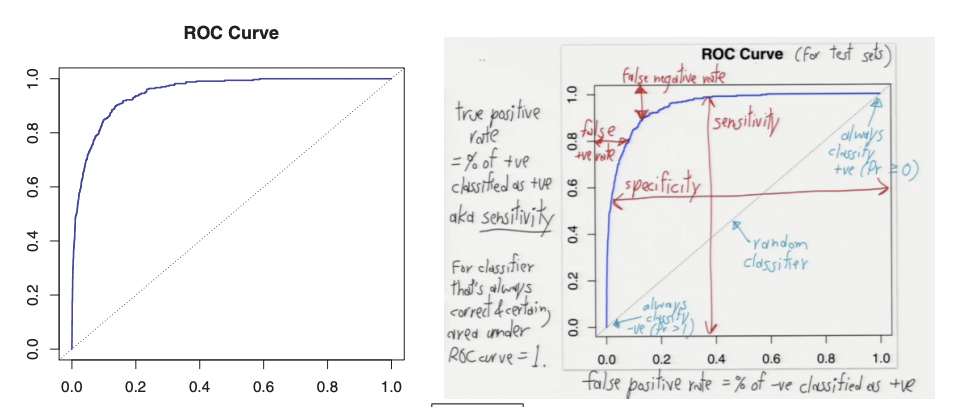
\includegraphics[width=\linewidth]{ROC.png}

\section{$\boxed{\text{Design Matrix}}$}
\settowidth{\MyLen}{\texttt{.begin.verbatim..} }
\begin{tabular}{@{}p{\the\MyLen}%
                @{}p{\linewidth-\the\MyLen}@{}}
Centering:         &  subtracting $\mu^\top$ from each row of $X$: $X \xrightarrow{}\dot X$\\
Decorrelating: & Applying rotation $Z = \dot X V$ where $\Var(X) = V \Lambda V^\top$. Covariance matrix of $Z$ is $\Lambda$ (diagonal)\\
Sphering: & $W = \dot X \Var(X)^{-1/2}$ ($\Sigma^{-1/2}$:ellipsoid to sphere)\\
Whitening: & Perform centering, and then sphering \\
\end{tabular}

\section{$\boxed{\text{Bias-Variance Tradeoff}}$}
Statistical Bias: $\E[\hat\theta-\theta]=\E[\hat\theta]-\theta$.

\textbf{Bias}: error due to inability of hypothesis $h$ to fit $g$ perfectly e.g., fitting quadratic $g$ with a linear $h$\\
\textbf{Variance}: error due to fitting random noise in data
e.g., we fit linear $g$ with a linear $h$, yet $h \neq g$.

Overfitting: Low Bias, High Variance \\
Underfitting: High Bias, Low Variance.

Adding a feature usually increases variance [don’t add a feature unless it reduces bias more]. Adding a feature results in a non-increasing bias. 

Forward/Backward stepwise selection aren't guaranteed to find optimal features. Backward stepwise selection looks at $d^{\prime}-1$ features at a time, where $d^{\prime}$ is current num of features (one at a time). Use Forward selection if we think few features important, Backward selection if many features important.

higher residuals $\implies$ higher bias\\
higher complexity $\implies$ higher variance

$\Var(h(z)) = E\left[(h(z)-E[h(z)])^{2}\right] \approx \sigma^2\frac d n$

\textbf{Bias-Variance Decomposition:} \\
$\begin{aligned}[t] \text{Model Risk} &=\E[L(h(z), \gamma)]
=\E[(h(z)-\gamma)^2] \\
&=\underbrace{(\mathrm{E}[h(z)]-g(z))^{2}}_{\text {bias}^{2} \text { of method }}+\underbrace{\operatorname{Var}(h(z))}_{\text {variance of method }}+\underbrace{\operatorname{Var}(\epsilon)}_{\text {irreducible error }}
\end{aligned}$ where $\mathrm{E}[\gamma]=g(z) ; \operatorname{Var}(\gamma)=\operatorname{Var}(\epsilon)$.

Note: the model determines Bias-Variance Tradeoff, not the algorithm used to solve the model/optimization problem.

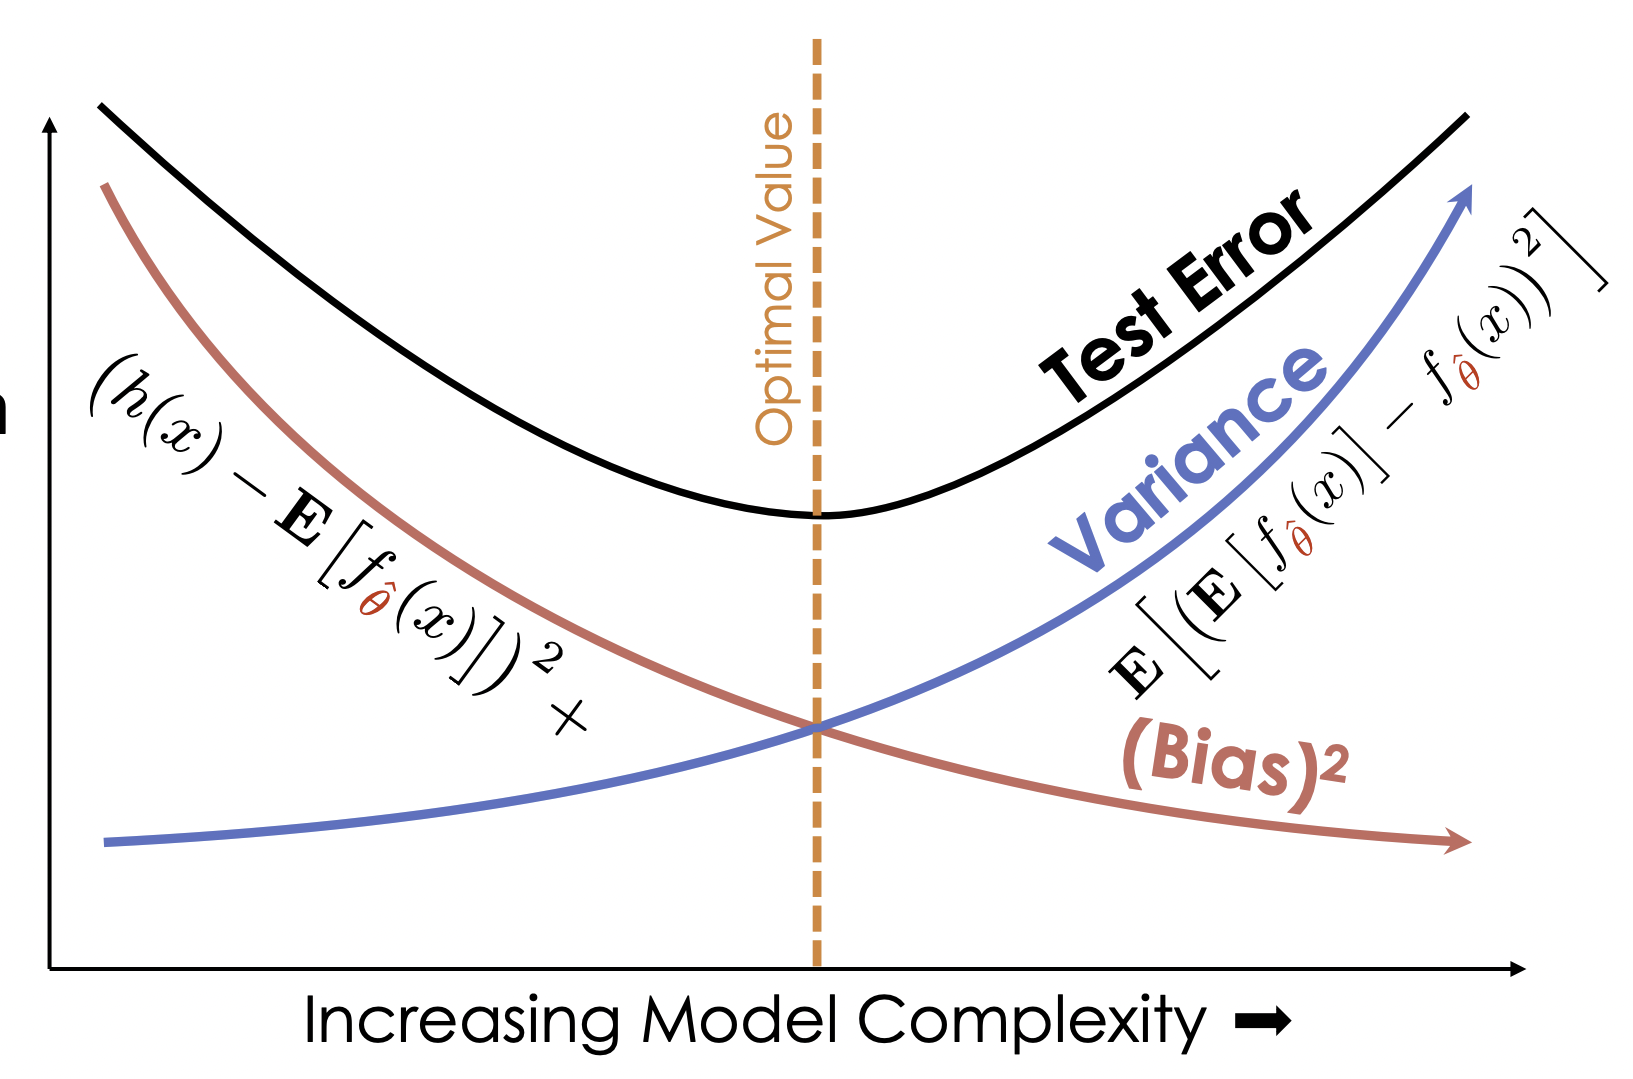
\includegraphics[height = 1.6 in]{Bias-Variance.png}

% todo add bias var tradeoff diagarm


\section{$\boxed{\text{Isocontour/Voronoi Diagrams}}$}
\begin{tabular}{@{}p{\linewidth/2-0.25cm}@{\hskip 0.5cm}@{}p{\linewidth/2-0.25cm}@{}}
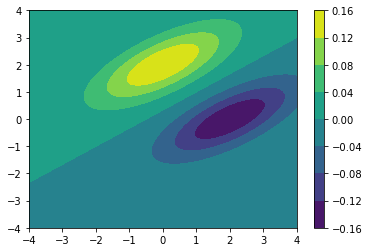
\includegraphics[width=\linewidth/6*5]{LDA.png} & 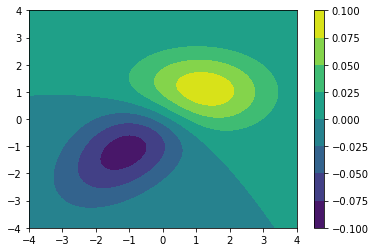
\includegraphics[width=\linewidth/8*7]{QDA_1.png} \\
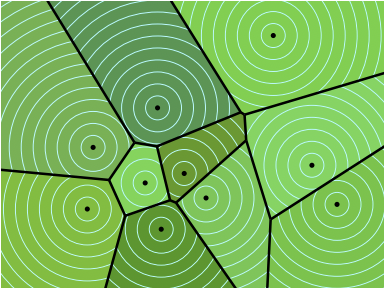
\includegraphics[width=\linewidth/6*5]{Voronoi_LDA.png} & 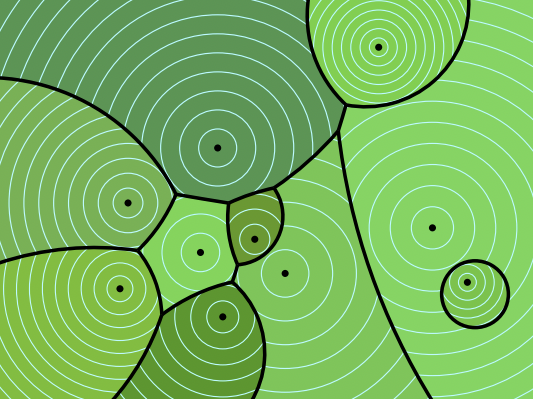
\includegraphics[width=\linewidth/6*5]{Voronoi_QDA.png} \\
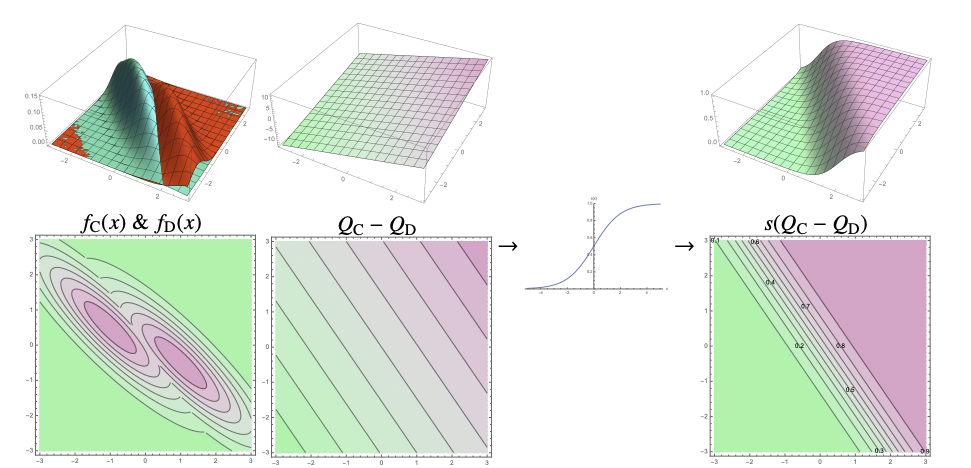
\includegraphics[width=\linewidth/8*7]{LDA_Isocontours.png} & 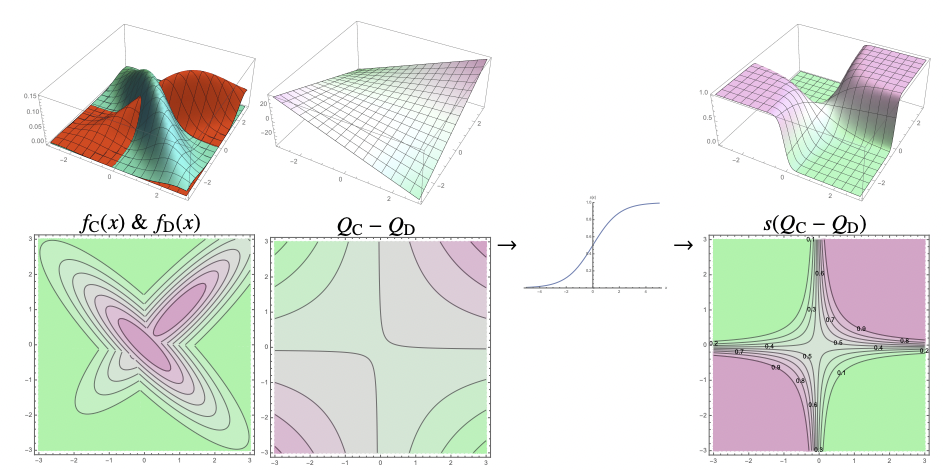
\includegraphics[width=\linewidth/8*7]{QDA_Isocontours.png} \\
 \textbf{LDA:} same variance; decision boundary is linear & \textbf{QDA:} different variance; decision boundary is curved towards class(es) w/ lower variance 
\end{tabular} \vspace{0.5em} 
\hrule \vspace{0.5em}
 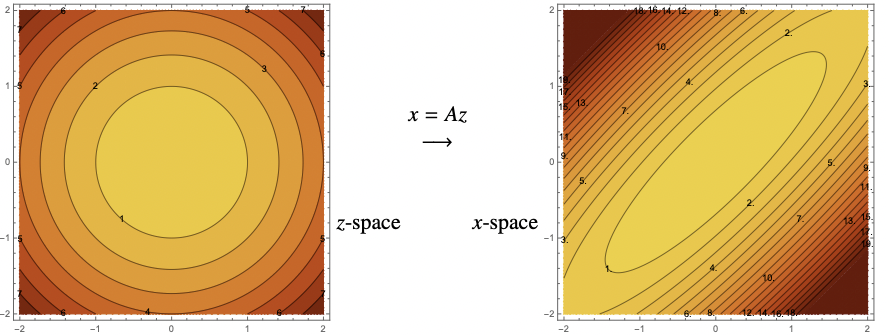
\includegraphics[height = 1 in]{Quadratic_Isosurface.png}
 
 Quadratic Form: $x^{\top}A^{-2}x = \| A^{-1}x\|_2^2$ is an ellipsoid with axes $v_1, v_2, \dots v_n$ (eigenvectors of $A$) and radii $\lambda_1, \lambda_2, \dots, \lambda_n$ (eigenvalues of $A$). Note that $A > 0$.
 
 Gaussian with covariance matrix $\Sigma = \frac{1}{n} \hat{X}^{\top} \hat{X}$ isocontours with radii of length $\sqrt{\lambda_i(\Sigma)} = \sigma_i(X)$

\section{$\boxed{\text{Decision Trees}}$}
Tree with each node denoting a split over some feature. Leaf node specifies class. 
deep decision tree = overfit = high variance \\
Calculate entropy (2 classes $C,D$): $H(S)=-\sum_{\mathrm{C}} p_{\mathrm{C}} \log _2 p_{\mathrm{C}}$ \\ 
$p_{\mathrm{C}}=\frac{\left|\left\{i \in S: y_i=\mathrm{C}\right\}\right|}{|S|}$.\\ Choose split that maximizes information gain $H(S)-H_{\mathrm{after}}=H(S)-\frac{\left|S_l\right| H\left(S_l\right)+\left|S_r\right| H\left(S_r\right)}{\left|S_l\right|+\left|S_r\right|}.$
\\
Classification: worst case $O(depth),$ often $O(\log n)$\\
Training: $O(nd),$ at each split point try $O(d)$ splits.\\
Regression: Leaf stores label $\mu_S=\frac{1}{|S|} \sum_{i \in S} y_i$\\
Cost $J(S)=\operatorname{Var}\left(\left\{y_i: i \in S\right\}\right)=\frac{1}{|S|} \sum_{i \in S}\left(y_i-\mu_S\right)^2$\\
Stop early: reasons: speed, pure leaves (i.e. complete alg) overfits. use: check node and use majority (mean for regression).\\
Pruning: greedily remove split whose removal improves validation performance. more reliable than stopping.\\
\textbf{Bagging:} run learning algorithm on random subsamples of training set (weak learner). regression: take average, class: take majority.\\
Minimize bias as much as possible - averaging reduces variance/overfit. Bagging worse for kNN.
% \tiny{Credits: Jonny Pei, Elden Ren, Jainil Shah, Rahul Shah}
\section{$\boxed{\text{Random Forests}}$}
At each node, take rnd sample of $m$ features (out of $d$).\\
Classification: $m_{\text{init}}\approx\sqrt d$
\\
Regression: $m_{\text{init}}\approx\frac d3$
\\
Smaller $m$ = less features = less complex model = more bias

\section{$\boxed{\text{Kernels}}$}
Can speedup algorithms such as SVMs, $k$NN, Regression (linear \& logistic), $k$-means, etc.
\\
$w = X^\top a = \sum_{i=1}^n a_i X_i$
Substitute this into the algorithm so we have to optimize $n$ weights $a$ instead of $d$ weights $w$ \\
\textbf{Kernel Ridge Regression}: Center $X$ and $y$ so means are 0, $X_{i, d+1} = 1$. Solve normal equations: $(X^\top X + \lambda I)w = X^\top y$\\
If $a$ is a solution to $(X^\top X + \lambda I) a = y$, $X^\top y = X^\top X X^\top a + \lambda X^\top a = (X^\top X + \lambda I) X^\top a \implies w = X^\top a$\\
The dual: $\min ||X X^\top a - y||^2 + \lambda ||X^\top a||^2$\\
Test phase: $h(z) = w^\top z = a^\top X z = \sum_{i=1}^n a_i(X_i^\top z)$, if $X_i^\top z$ are precomputed, it takes $O(n)$ time to evaluate $h$ vs $O(d)$ time for primal method. \\
kernel fn: $k(x, z) = x^\top z$, kernel mtx: $K = X X^\top$ ($K_{ij} = k(X_i, X_j)$)\\
kernel matrix must be PSD + symmetric
\\
Solve $(K+\lambda I)a=y$ $O(n^3)$, test $h(z) = \sum a_i k(X_i, z)$ $O(nd)$ time \\
Dual: $O(n^3 + n^2 d)$, Primal: $O(d^3 + d^2 n)$, dual is better when $d>n$.\\
\textbf{Kernel Trick}: Polynomial kernel = $k(x, z) = (x^\top z + 1)^p$ \\ Gaussian kernel = $k(x, z)=\exp \left(-\frac{\|x-z\|^2}{2 \sigma^2}\right)$\\
Can compute $k(x, z) = \Phi(x)^\top \Phi(z)$ in $O(d)$ time instead of $O(d^p)$\\
Enables us to implicitly handle polynomial features efficiently \\
\textbf{Kernel Perceptrons}:\\
$w \leftarrow y_1 \Phi(X_1)$: while some $y_i \Phi(X_i) \cdot w < 0$, $w \leftarrow w + \epsilon y_i \Phi(X_i)$ \\
for each test pt $z$, $h(z) \leftarrow w \cdot \Phi(z)$\\
Let $\Phi(X)$ be $x \times D$ matrix with rows $\Phi(X_i)^\top$ \\
Dualize with $w = \Phi(X)^\top a$, $a_i \leftarrow a_i + \epsilon y_i$, $h(z) = \sum_{i=1}^n a_j + k(X_{ij}, z)$ \\
$\Phi(X_i) \cdot w = (\Phi(X) w)_i = (\Phi(X) \Phi(X)^\top a)_i = (Ka)_i$\\
$a \leftarrow \begin{bmatrix}
y_1 & 0 & \cdots & 0
\end{bmatrix}^\top$: while some $y_i(Ka)_i < 0$, $a_i \leftarrow a_i + \epsilon y_i$\\
$O(n^2 d)$ to kernel mtx $O(1)$ to update $a$, $O(n)$ to update $Ka$

\section{$\boxed{\text{Learning Theory}}$}
Range Space (P, H):
P = set of all possible train/test pts (ex. $\mathbb R^d$)
\\
H = set of all possible hypotheses
Dichotomy: split of input data into two separate classes, not necessarily linear decision boundary. 
Shatter Function: $\Pi_H(X)=|\{X\cap h:h\in H\}|$ = maximum number of dichotomies hypothesis class $H$ can produce in particular set of points $X$.
$\displaystyle\Pi_{H}(n)=\max _{|X|=n, X \subseteq P} \Pi_{H}(X)$= maximum number of dichotomies hypothesis class $H$ can produce amongst a set of $n$ data points and is only ever $2^n$ (known as shattering) or polynomial in $n$.

VC Dimension = the largest number of points $D$ s.t. $\Pi_H(D) = 2^n$. Basically largest number of points a hypothesis class can produce all dichotomies of. Can be infinite, can be $0$.
A linear perceptron classifier with $d$ parameters ($d$-dimensional weight vectors) has a VC dimension of $d$. For example, 2$d$ linear perceptron (three weights - one for each dimension and one fictitious dimension = bias) has VC dimension of 3.

\section{$\boxed{\text{AdaBoost}}$}
Ensemble method that trains multiple learns on weighted sample points and weights learner. (misclassified points = increased weights, accurate learners = increased weights). Find classifier $G_T$ and coefficient $\beta_T$ to minimize\\
$\text{Risk} = \frac{1}{n} \sum_{i=1}^n L(M(X_i), y_i)$ with $M(X_i) = \sum_{t=1}^T \beta_t G_t(X_i)$\\ 
AdaBoost metalearner uses $L(\rho, \ell) = e^{-\rho \ell}$
$w_i^{(T + 1)} = w_i^{(T)} \exp(-\beta_T \, y_i \, G_T(X_i))$, $\beta_T = \frac{1}{2}\ln \bigg(\frac{1 - \mathrm{err}_T}{\mathrm{err}_T}\bigg)$
$\mathrm{err}_T = \frac{\sum_{y_i \neq G_T(X_i)}w_i^{(T)}}{\sum_{i = 1}^n w_i^{(T)}}.$ metalearner: $h(z) = \mathrm{sign}(\sum_{t=1}^T \beta_t G_t(z))$\\
AdaBoost reduces bias, but effect on variance is hard to figure out (may sometimes overfit).
\section{$\boxed{\text{Neural Nets}}$}
Multi-layered perceptron, each layer puts outputs of previous layer linear function and then activation function. Minimize loss via gradient descent \\
Naive: $O(e^2)$, Backprop: $O(e).$\\
Solve vanishing gradient problem: use ReLU activation $r(\gamma)=\max \{0, \gamma\}$
Softmax activation: $
z_i(t)=\frac{e^{t_i}}{\sum_{j=1}^k e^{t_j}};z_i \in(0,1) ; \sum_{i=1}^k z_i=1$\\ Use cross entropy instead of squared loss; $k$-class softmax output, cross-entropy: $L(z, y)=-\sum_{i=1}^k y_i \ln z_i$ \\ $\nabla_W L=(z-y) h^{\top},$ $
\nabla_h L =W^{\top}(z-y)
$\\
CNNs: local connectivity and filter - perform convolution of small patches of image.
\section{$\boxed{\text{Principal Component Analysis}}$}
Goal: find directions with highest variance\\
Sol: Use SVD to decompose matrix and find eigenvectors for greatest singular values; same as finding Rayleigh quotients.\\
Low-rank approximation is lossy feature selection: you lose lower variance components yet select out low-singular values (often ``noise" components)
% \\
% $XX^\top$

\section{$\boxed{\text{Clustering}}$}
NP-hard: find $\argmin_y \sum_{i=1}^k \sum_{y_j=i} ||X_j -\mu_i||^2$\\
K-means: alternate between fixed $y_j$'s update $\mu_i$'s and vice versa. Halt when step 2 changes no assignments. Both steps decrease objective fn unless they change nothing; alg must terminate.\\
Initialization: Forgy method (choose $k$ random points to be centroids). Can also use the (worse) random partitions - randomly assign each point to a cluster.
K-medioids: K-means, but instead of using mean, use medioid, sample point minimizing total distance to other points in cluster.\\
Hierarchical clustering: creates a tree, every subtree is a cluster. Bottom-up (agglomerative) start with each point a cluster; repeatedly fuse pairs minimizing $d(A, B)$. Linkage functions: \\
complete: $d(A, B) = \max \{ d(w, x) : w \in A, x \in B \}$\\
single: $d(A, B) = \min \{d(w, x): w \in A, x \in B \}$\\
average:  $d(A, B) = \frac{1}{|A||B|}\sum_{w \in A} \sum_{x \in B} dist(w, x)$\\
centroid: $d(A, B) = dist(\mu_A, \mu_B)$\\
Top-down (divisive) starts with single cluster, repeatedly splits

\section{$\boxed{\text{Miscellaneous}}$}
NP-Hard to find optimal linear classifier
\begin{tabular}{@{}p{\the\MyLen}%
                @{}p{\linewidth-\the\MyLen}@{}}
Bayes vs. GDA & Bayes uses true mean/variance, while GDA uses sample mean/variance. True mean/variance equal $\not \Rightarrow$ Sample mean/variance equal\\

Cauchy-Schwarz &  $|\langle x, y \rangle | \leq \| x \| \cdot \| y \|$  \\
Unique Optimum & Only ridge regression has one unique optimum (not Least Squares, Lasso, or Logistic).\\
Training Data: & Training on less data can improve train acc, training on more data can improve val/test acc.\\
\end{tabular}
\tiny{Credits: Jonny Pei, Elden Ren, Jainil Shah, Rahul Shah}
\end{multicols}
%$\ln(ab)=\ln(a)+\ln(b);\quad a^{x+y}=a^x\cdot a^y$
\end{document}
